\documentclass[a4paper,11pt]{article}
\usepackage{lecturenotes}
\usetikzlibrary{matrix}
\lectureheader{ELE734}{4}
\begin{document}
\tableofcontents
\clearpage
\noteheading{1}{Delay}
\noteheading{2}{Elmores Delay}
\keyequation{$T_{pd}$, Time to Discharge $C_{i}$}{t_{pd} = \sum_i R_{i}C_{i}}
\par\addvspace{7pt}
\noindent\begin{minipage}{\linewidth}
    \centering
    \captionsetup{hypcap=false,type=figure}
    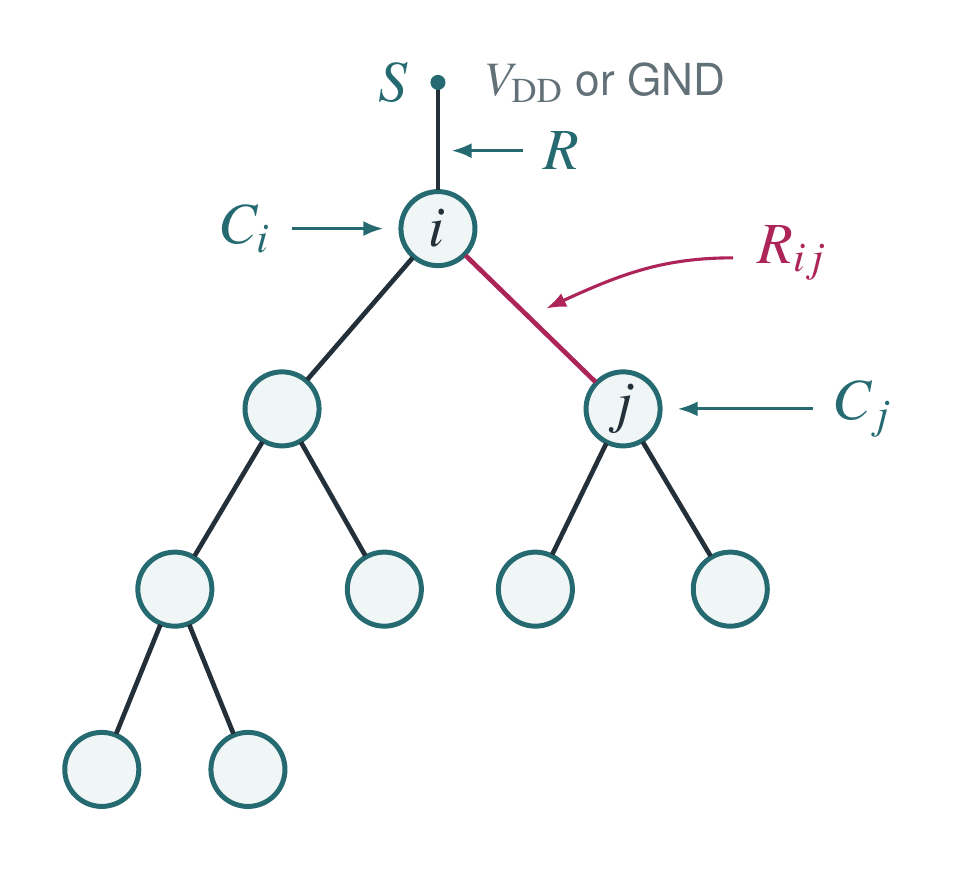
\includegraphics[width=0.5\linewidth,keepaspectratio]{figures/elmore-rc-tree.png}
    \caption{Elmore RC Tree}
    \label{fig:}
\end{minipage}
\par\addvspace{7pt}

\noindent\begin{minipage}{\linewidth}
    \begin{notepanels}[gap=8mm]
        \begin{notepanel}{}
            \begin{notecircuit}[american,scale=0.55,transform shape]
                {Single-capacitor discharge}
                \draw (0,1.1) node[ground] {} -- (0,1.6)
                    to[R,l=$R$] (2.1,1.6)
                    to[C,l=$C_i$] (2.1,0) node[ground] {};
            \end{notecircuit}
            \centering\small
            Initially $v_{C_i}(0)=V_{DD}$; discharge toward $0$.
            \[t_{pd}=RC_i\]
        \end{notepanel}
        \begin{notepanel}{}
            \begin{notecircuit}[american,scale=0.55,transform shape]
                {Two-capacitor discharge}
                \draw (0,1.1) node[ground] {} -- (0,1.6)
                    to[R,l=$R_1$] (2.1,1.6) coordinate (c1)
                    to[R,l=$R_2$] (4.2,1.6)
                    to[C,l=$C_2$] (4.2,0) node[ground] {};
                \draw (c1) node[circ] {}
                    to[C,l=$C_1$] (2.1,0) node[ground] {};
            \end{notecircuit}
            \centering\small
            Initially $v_{C_1}(0)=v_{C_2}(0)=V_{DD}$;\\
            both capacitors discharge toward $0$.
        \end{notepanel}
    \end{notepanels}

    {\small Each capacitance is weighted by the resistance shared by its
    path to ground and the observed node's path to ground.\par}

    \begin{notepanels}[gap=8mm]
        \begin{notepanel}{}
            \begin{notederivation}{Discharge delay at $C_2$}
                t_{pd,C_2} &= R_1C_1+(R_1+R_2)C_2 \\
                    &= (R_1+R_2)C_2
                        +\underbrace{R_1C_1}_{\text{correction term}}
            \end{notederivation}
        \end{notepanel}
        \begin{notepanel}{}
            \begin{notederivation}{Discharge delay at $C_1$}
                t_{pd,C_1} &= R_1C_1+R_1C_2 \\
                    &= R_1(C_1+C_2)
            \end{notederivation}
        \end{notepanel}
    \end{notepanels}
\end{minipage}
\notedefinition{Finding Delay through Resistance and Capacitance}{
    \begin{enumerate}
        \item Find all the resistance that a target capacitance will discharge through
        \item Only use resistances to calculate the delay contribution of all capacitances
    \end{enumerate}
}
\noteheading{3}{Effective Resistance}
\par\addvspace{7pt}
\noindent\begin{minipage}{\linewidth}
    \centering
    \captionsetup{hypcap=false,type=figure}
    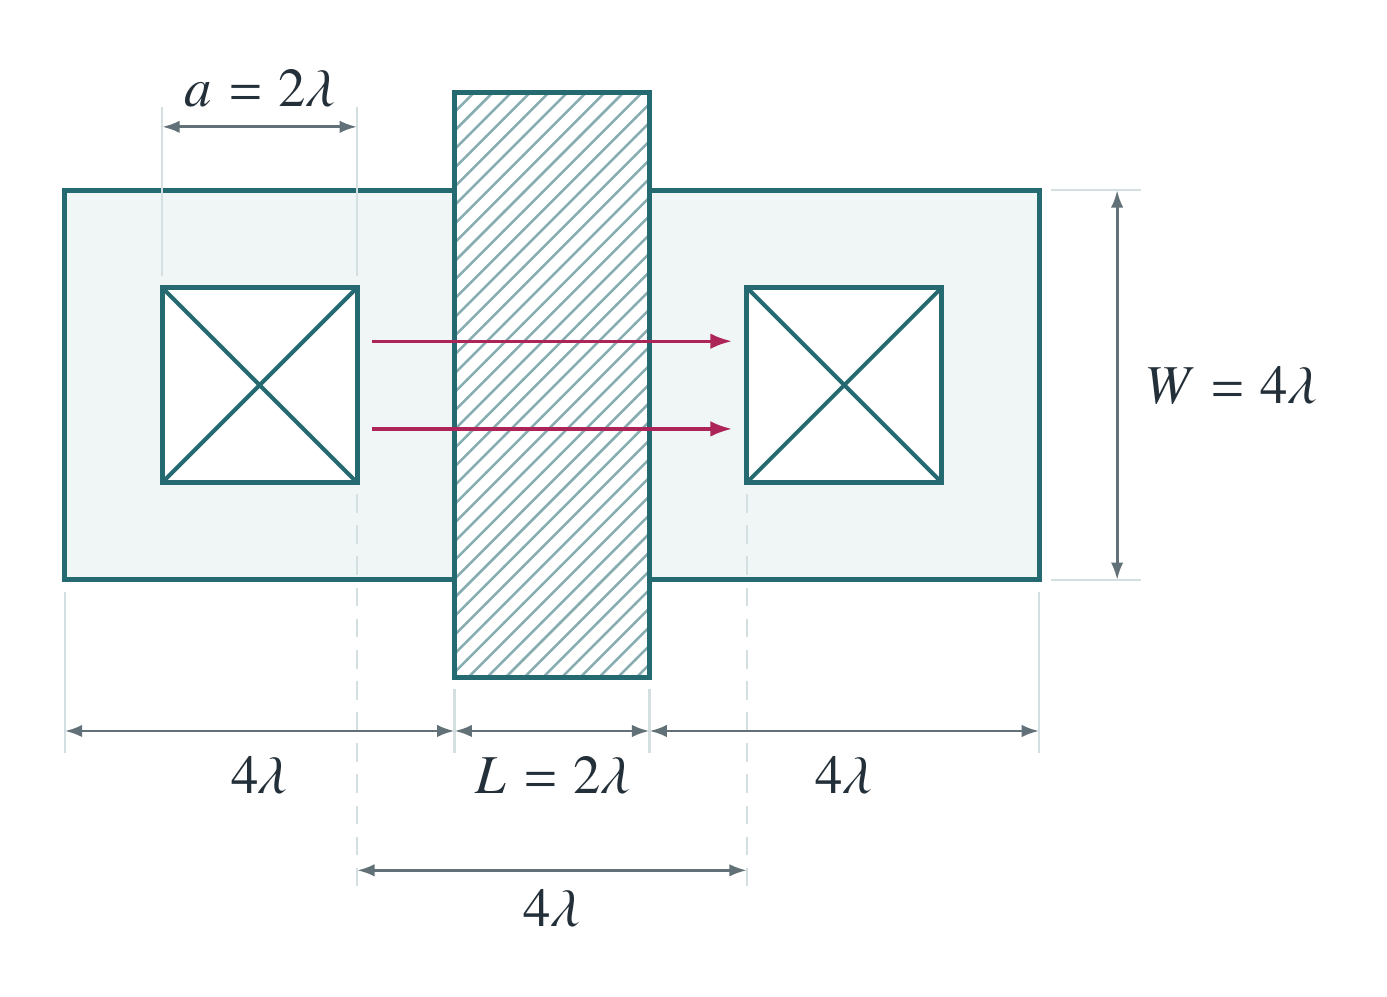
\includegraphics[width=0.5\linewidth,keepaspectratio]{figures/unit-mos-transistor.png}
    \caption{Unit MOSFET Device}
    \label{fig:}
\end{minipage}
\par\addvspace{7pt}

A unit transistor is the \textit{smallest transistor that can be built with contact to metal} and is $\approx 8\lambda \times 12 \lambda$
\begin{notetable}{lX}{\textbf{Device Type} & \textbf{K Times of Unit Width ($4\lambda$)}}
     NMOS & $\frac{R}{k}$ \\
     PMOS & $\frac{2R}{k}$ \\
\end{notetable}
\noindent\begin{minipage}{\linewidth}
\noteheading{3}{Equivalent RC Circuit}
    \begin{notepanels}[gap=6mm]
        \begin{notepanel}{}
            \begin{notecircuit}[american,scale=0.55,transform shape,
                font=\large]{NMOS equivalent RC model}
                \path[use as bounding box] (-1.5,-3.8) rectangle (10.6,4.2);
                \node[nmos] (nrc) at (0,0) {$k$};
                \draw (nrc.G) -- ++(-0.35,0) node[ocirc] {}
                    node[left] {$g$};
                \draw (nrc.D) -- ++(0,0.35) node[ocirc] {}
                    node[above] {$d$};
                \draw (nrc.S) -- ++(0,-0.25) node[ground] {}
                    node[left=3pt] {$s$};
                \node[NoteAccent] at (1.35,0) {$\Longrightarrow$};

                \draw (2.7,0.7) node[ocirc] {} node[above] {$g$}
                    to[C,l=$kC$] (2.7,-0.9) node[ground] {};

                \draw (5,1.5) node[circ] {} node[above] {$d$}
                    to[R,l_=$R/k$] (5,0)
                    to[nos] (5,-1.5) node[circ] {}
                    node[left] {$s$} -- (5,-1.8) node[ground] {};
                \draw (5,1.5) -- (6.5,1.5)
                    to[C,l=$kC$] (6.5,-0.1) node[ground] {};
                \draw (5,-1.5) -- (6.5,-1.5)
                    to[C,l=$kC$,color=NoteAccent]
                    (6.5,-3.1) node[ground] {};
                \draw[NoteAccent,line width=0.3pt,
                    -{Latex[length=2pt,width=1.4pt]}]
                    (7.9,-2.9) -- (7.4,-2.9) -- (6.9,-2.5);
                \node[anchor=west,align=left,font=\normalsize\sffamily,
                    text=NoteAccent] at (8,-2.95)
                    {Not relevant\\to delay};
            \end{notecircuit}
        \end{notepanel}
        \begin{notepanel}{}
            \begin{notecircuit}[american,scale=0.55,transform shape,
                font=\large]{PMOS equivalent RC model}
                \path[use as bounding box] (-1.5,-3.8) rectangle (10.6,4.2);
                \node[pmos] (prc) at (0,0) {$k$};
                \draw (prc.G) -- ++(-0.35,0) node[ocirc] {}
                    node[left] {$g$};
                \draw (prc.S) -- ++(0,0.25) node[vcc] {$V_{DD}$};
                \node[left=3pt] at (prc.S) {$s$};
                \draw (prc.D) -- ++(0,-0.35) node[ocirc] {}
                    node[below] {$d$};
                \node[NoteAccent] at (1.35,0) {$\Longrightarrow$};

                \draw (2.7,-0.9) node[ocirc] {} node[below] {$g$}
                    to[C,l_=$kC$] (2.7,0.7) node[vcc] {$V_{DD}$};

                \draw (5,1.5) node[circ] {} node[left] {$s$}
                    to[R,l_=$2R/k$] (5,0)
                    to[nos] (5,-1.5) node[circ] {} node[left] {$d$};
                \draw (5,1.5) -- (5,1.8) node[vcc] {$V_{DD}$};
                \draw (5,1.5) -- (6.5,1.5)
                    to[C,l_=$kC$,color=NoteAccent]
                    (6.5,3.1) node[vcc] {$V_{DD}$};
                \draw (5,-1.5) -- (6.5,-1.5)
                    to[C,l=$kC$] (6.5,-3.1) node[ground] {};
                \draw[NoteAccent,line width=0.3pt,
                    -{Latex[length=2pt,width=1.4pt]}]
                    (7.9,1.85) -- (7.4,1.85) -- (6.9,2.15);
                \node[anchor=west,align=left,font=\normalsize\sffamily,
                    text=NoteAccent] at (8,1.6)
                    {Not relevant\\to delay};
            \end{notecircuit}
        \end{notepanel}
    \end{notepanels}
    {\small\color{NoteAccent}
    Constant voltages such as $V_{DD}$, can be treated as GND for delay calculations because $dV_{\mathrm{const}}/dt=0$.\par}
\end{minipage}
\noteheading{3}{Delay of an Inverter}



\noindent\begin{minipage}{\linewidth}
    \begin{notecircuit}[american,scale=0.55,transform shape,
        font=\large]{CMOS inverter}
        \node[pmos] (delay-p) at (0,0.85) {$2$};
        \node[nmos] (delay-n) at (0,-0.85) {$1$};
        \draw (delay-p.G) -- (delay-n.G) coordinate[midway] (delay-in);
        \draw (delay-in) -- ++(-0.45,0) node[ocirc] {} node[left] {$A$};
        \draw (delay-p.D) -- (delay-n.D) coordinate[midway] (delay-out);
        \draw (delay-p.S) -- ++(0,0.25) node[vcc] {$V_{DD}$};
        \draw (delay-n.S) -- ++(0,-0.25) node[ground] {};
        \draw (delay-out) node[circ] {} -- (1.9,0) node[circ] {}
            node[above] {$Y$}
            to[C,l=$xC$] (1.9,-1.6) node[ground] {};
    \end{notecircuit}

    \newcommand{\inverterdelayrc}[3]{%
        \path[use as bounding box] (-2.8,-5.1) rectangle (4.4,5.8);
        \draw (0,3) node[circ] {}
            to[R,l=$R$] (0,1.5)
            to[#1] (0,0) node[circ] {}
            to[R,l=$R$] (0,-1.5)
            to[#2] (0,-3) node[circ] {};
        \draw (0,3) -- (0,3.3) node[vcc] {$V_{DD}$};
        \draw (0,-3) -- (0,-3.3) node[ground] {};
        \draw (-1.7,0) node[circ] {} -- (3,0);
        \node[above,NoteAccent] at (1.5,0) {$Y=#3$};
        \draw (-1.7,0) to[C,l=$2C$]
            (-1.7,1.6) node[vcc] {$V_{DD}$};
        \draw (-1.7,0) to[C,l_=$C$]
            (-1.7,-1.6) node[ground] {};
        \draw (3,0) to[C,l=$xC$] (3,-1.6) node[ground] {};
        \draw[NoteMuted] (0,3) -- (1.7,3)
            to[C,l_=$2C$] (1.7,4.6) node[vcc] {$V_{DD}$};
        \draw[NoteMuted] (0,-3) -- (1.7,-3)
            to[C,l=$C$] (1.7,-4.6) node[ground] {};
        \draw[NoteAccent,line width=0.45pt]
            (1.3,3.5) -- (2.1,4.1)
            (1.3,-4.1) -- (2.1,-3.5);
    }
    \begin{notepanels}[gap=8mm]
        \begin{notepanel}{}
            \begin{notecircuit}[american,scale=0.55,transform shape,
                font=\large]{Initially: $A=0$, $Y=1$}
                \inverterdelayrc{ncs}{nos}{1}
            \end{notecircuit}
        \end{notepanel}
        \begin{notepanel}{}
            \begin{notecircuit}[american,scale=0.55,transform shape,
                font=\large]{Falling transition: $A=1$, $Y:1\to0$}
                \inverterdelayrc{nos}{ncs}{1\to0}
            \end{notecircuit}
        \end{notepanel}
    \end{notepanels}
    {\small\color{NoteAccent}
    Crossed-out source capacitances are at fixed supply voltages and do not
    contribute to delay.\par}

    \begin{notecircuit}[american,scale=0.55,transform shape,
        font=\large]{Simplified RC circuit for the falling transition}
        \draw (0,1.6) -- (5.7,1.6);
        \draw (0,0) -- (5.7,0);
        \draw (0,1.6) node[circ] {} node[above] {$Y$}
            to[R,l_=$R$] (0,0);
        \draw (1.9,1.6) to[C,l=$2C$] (1.9,0);
        \draw (3.8,1.6) to[C,l=$C$] (3.8,0);
        \draw (5.7,1.6) to[C,l=$xC$] (5.7,0);
        \draw (2.85,0) -- (2.85,-0.25) node[ground] {};
    \end{notecircuit}
    \begin{notederivation}{Falling propagation delay}
        t_{pdf} &= R(2C+C+xC) \\
            &= (3+x)RC
    \end{notederivation}
\end{minipage}
\noteheading{4}{Fastest Logic Block}
The fastest logic gate is the fastest inverter.
\notedefinition{Faster Logic Block}{A inverter without any load}
\keyequation{Unloaded Inverter TPD}{\operatorname{tpdf}=\frac{\operatorname{tpdf}^{'}}{\operatorname{tpdf}^{''}} = \frac{(3+x)RC}{3RC} = 1 + \frac{x}{3} = \operatorname{tpdr}}

\notebox{Delay Normalization}{The unloaded $\operatorname{tpdf}^{''}$ is the value that is used to normalize when doing delay calculations}

\noteheading{4}{Bigger Inverter?}

\keyequation{Fall and Rise of a General Inverter}{\operatorname{tpdr} = \operatorname{tpdf} = 1 + \frac{x}{3W}}
\begin{notetable}{lX}{\textbf{Symbol} & \textbf{Meaning}}
     tpdf & Propogation delay fall time \\
     tpdr & Propogation delay rise time \\
     $x$ & Process Independent Value or Load \\
     $3W$ & Transistor Size \\
\end{notetable}

\par\addvspace{7pt}
\noindent\begin{minipage}{\linewidth}
    \centering
    \captionsetup{hypcap=false,type=figure}
    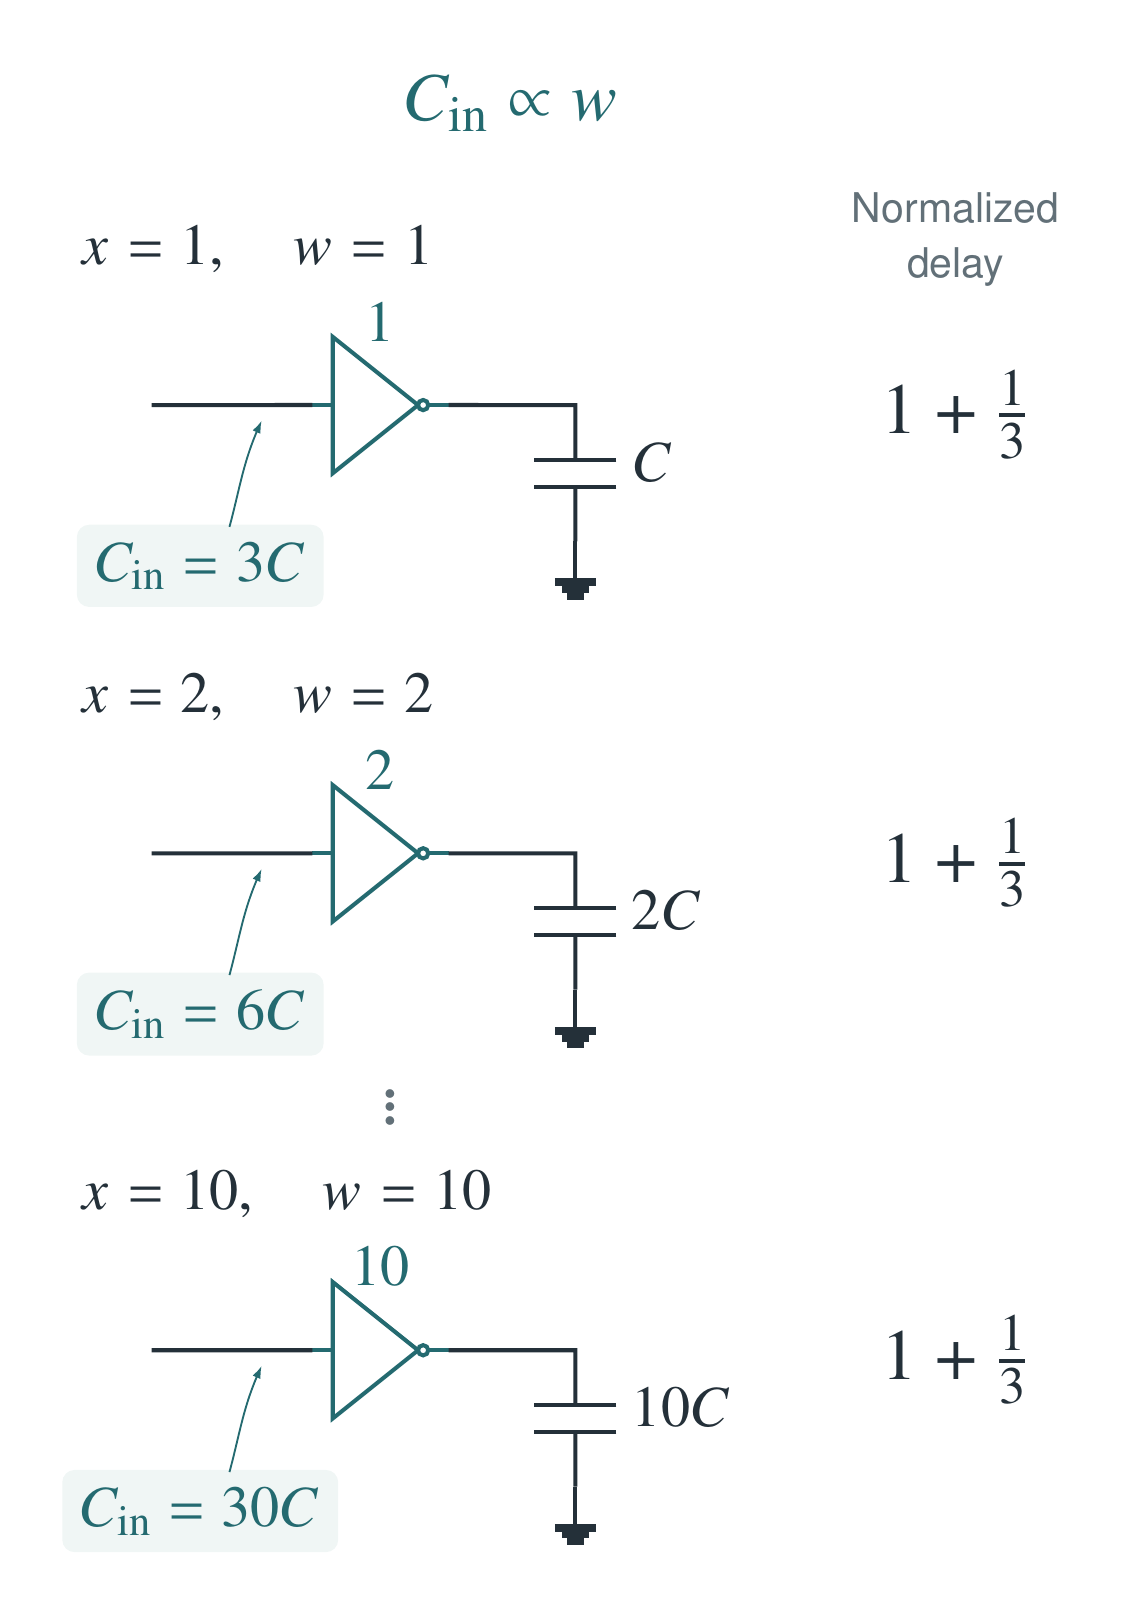
\includegraphics[width=0.6\linewidth,keepaspectratio]{figures/inverter-capacitance-scaling.png}
    \caption{Capacitance Scaling}
    \label{fig:}
\end{minipage}
\par\addvspace{7pt}
\keyequation{Output-Input Ratio}{h^{'} = \frac{w}{h}}
To maintain the same delay, we want $h^{'} = \frac{1}{3}$ (Input capacitance should 3 times bigger than output capacitance) 

\par\addvspace{7pt}
\noindent\begin{minipage}{\linewidth}
    \centering
    \captionsetup{hypcap=false,type=figure}
    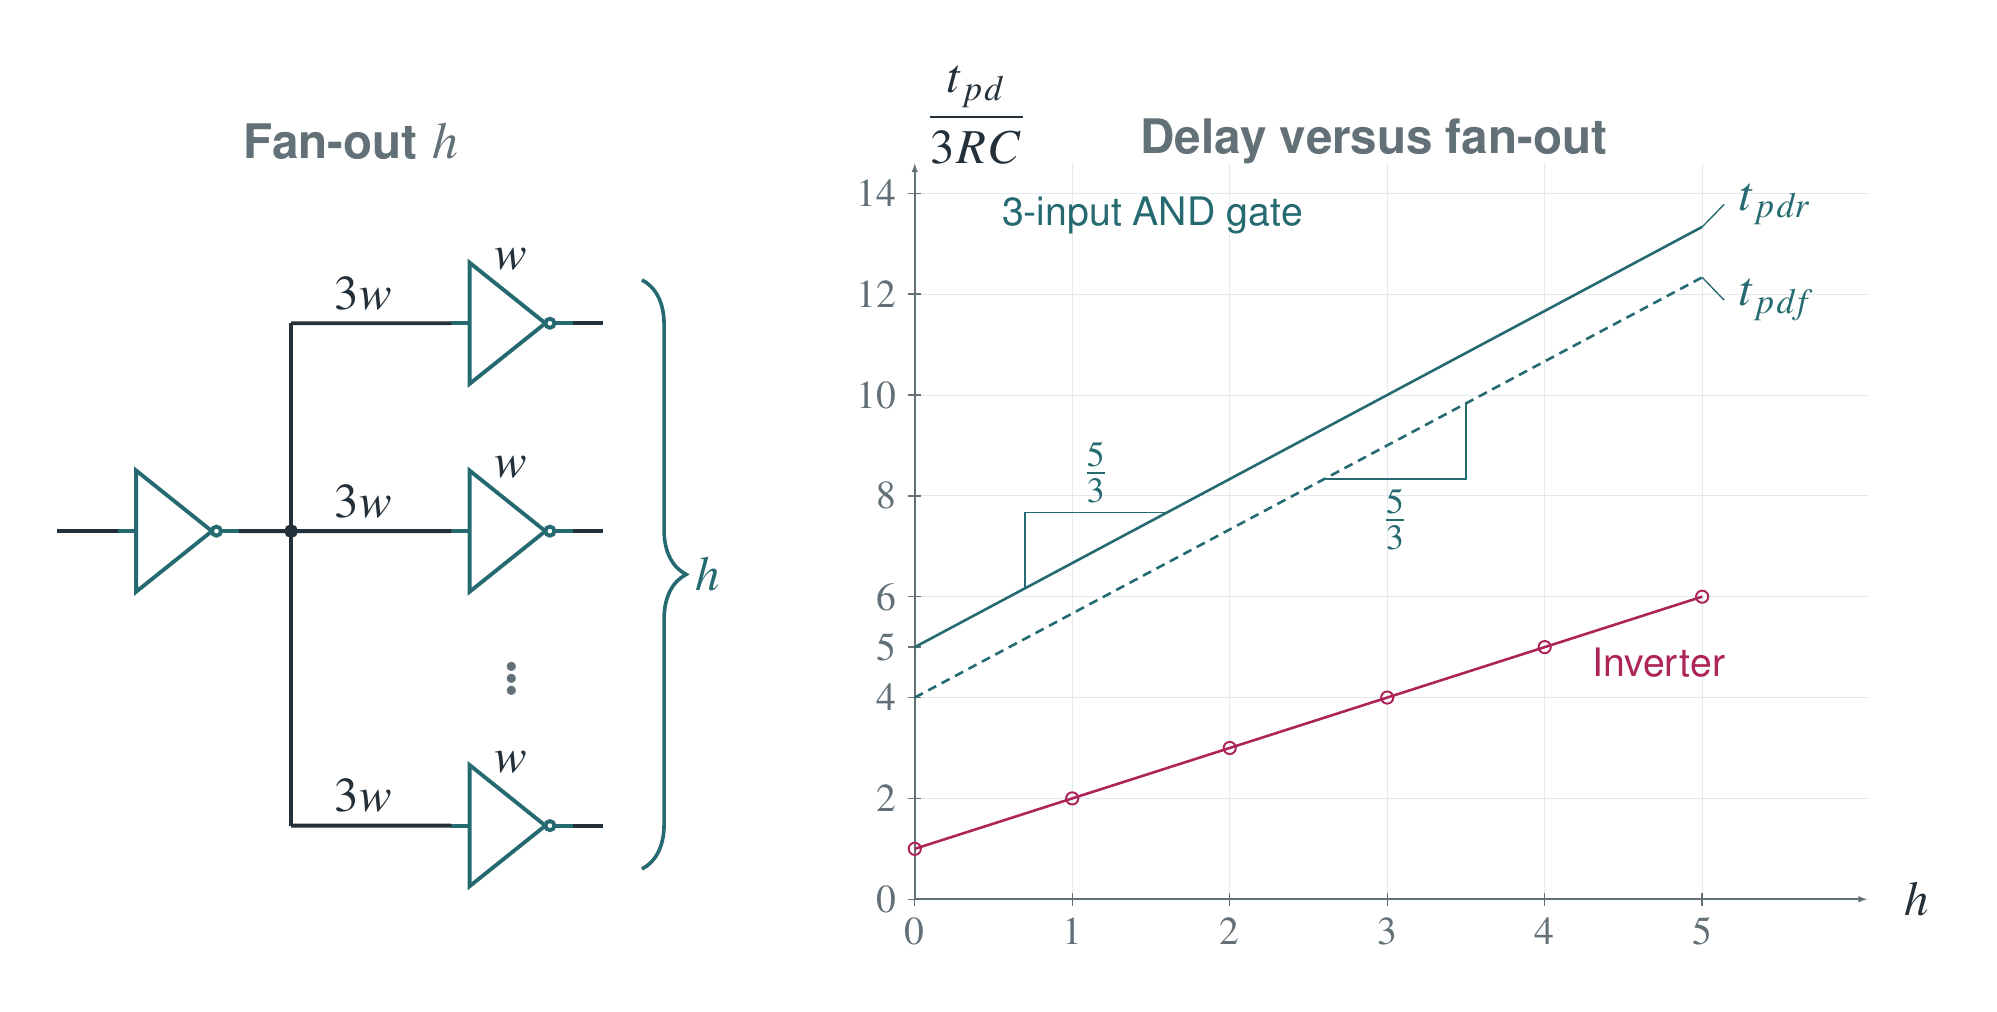
\includegraphics[width=0.6\linewidth,keepaspectratio]{figures/fanout-delay-comparison.png}
    \caption{Fanout Delay}
    \label{fig:}
\end{minipage}
\par\addvspace{7pt}
\par\addvspace{7pt}
\noindent\begin{minipage}{\linewidth}
    \centering
    \captionsetup{hypcap=false,type=figure}
    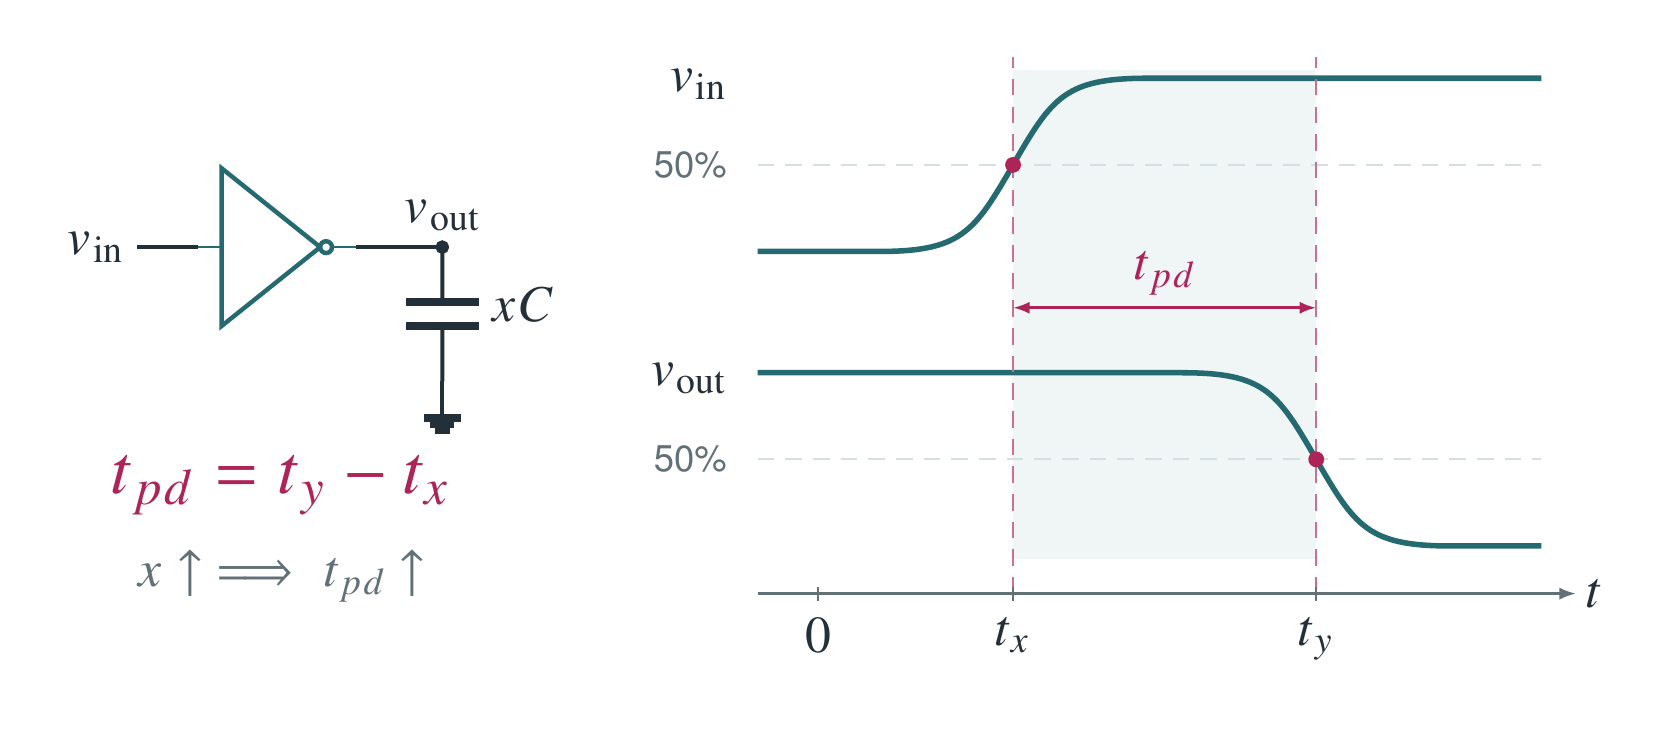
\includegraphics[width=0.8\linewidth,keepaspectratio]{figures/logic-cell-propagation-delay.png}
    \caption{}
    \label{fig:}
\end{minipage}
\par\addvspace{7pt}

\begingroup
\definecolor{DelayArrow}{HTML}{9C2F61}
\tikzset{
    delay-label/.style={font=\footnotesize\sffamily,text=NoteInk,
        align=center,inner sep=1pt},
    delay-arrow/.style={draw=DelayArrow,line width=0.45pt,
        -{Latex[length=2.6pt,width=1.8pt]},shorten <=3pt,shorten >=3pt},
    delay-terms/.style={matrix of math nodes,ampersand replacement=\&,
        nodes={font=\Large,inner sep=0pt,outer sep=0pt,anchor=base},
        inner sep=0pt,column sep=0pt}
}
\keyequation{Derivation of TPDR For H-identical Inverters (Fan-out of H)}{
    \begin{tikzpicture}[baseline=(inv-delay-1-2.base)]
        \node[inner sep=0pt] at (0,1.9)
            {$\displaystyle \operatorname{tpdr}=\operatorname{tpdf}
                =1+\frac{x}{3w}=1+\frac{3wh}{3w}$};
        \matrix (inv-delay) [delay-terms] at (0,0) {
            {}={} \& 1 \& {}+{} \& 1 \& {}\cdot{} \& h \\
        };
        \node[delay-label] (inv-logic) at (-1.8,0.95) {Logic effort};
        \node[delay-label] (inv-fanout) at (1.8,0.95) {Fan-out};
        \node[delay-label] (inv-intrinsic) at (-1.8,-0.9) {Intrinsic delay};
        \node[delay-label] (inv-electric) at (1.8,-0.9) {Electric effort};
        \draw[delay-arrow] (inv-logic.south)
            to[out=-90,in=90] (inv-delay-1-4.north);
        \draw[delay-arrow] (inv-fanout.south)
            to[out=-90,in=90] (inv-delay-1-6.north);
        \draw[delay-arrow] (inv-intrinsic.north)
            to[out=90,in=-90] (inv-delay-1-2.south);
        \draw[delay-arrow] (inv-electric.north)
            to[out=90,in=-90] (inv-delay-1-6.south);
    \end{tikzpicture}
}
\keyequation{Logical Effort Delay}{
    \begin{tikzpicture}[baseline=(general-delay-1-1.base)]
        \matrix (general-delay) [delay-terms] at (0,0) {
            d \& {}={} \& p \& {}+{} \& g \& h \\
        };
        \node[delay-label] (general-intrinsic) at (-2,1.05)
            {Intrinsic delay\\= parasitic delay};
        \node[delay-label] (general-electric) at (2,1.05) {Electric effort};
        \node[delay-label] (general-normalized) at (-2,-1.05)
            {Normalized delay\\$t_{pd}/(3RC)$};
        \node[delay-label] (general-logic) at (2,-1.05) {Logic effort};
        \draw[delay-arrow] (general-intrinsic.south)
            to[out=-90,in=90] (general-delay-1-3.north);
        \draw[delay-arrow] (general-electric.south)
            to[out=-90,in=90] (general-delay-1-6.north);
        \draw[delay-arrow] (general-normalized.north)
            to[out=90,in=-90] (general-delay-1-1.south);
        \draw[delay-arrow] (general-logic.north)
            to[out=90,in=-90] (general-delay-1-5.south);
    \end{tikzpicture}
}
\endgroup

\noindent\begin{minipage}{\linewidth}
\noteheading{2}{Delay in Multi-stage Logic Networks}
    % Keep the equation box whole inside this unbreakable minipage.
    \tcbset{noteblock/.append style={unbreakable,after skip balanced=9pt}}
    \begin{notecircuit}[american,scale=0.55,transform shape,
        font=\large]{Choose the gate input capacitances $x,y,z$ to minimize delay}
        \node[not port] (path-inv1) at (0,0) {};
        \node[nor port] (path-nor) at (3,0) {};
        \node[nand port] (path-nand) at (6,0) {};
        \node[not port] (path-inv2) at (9,0) {};
        \draw (path-inv1.in) -- ++(-0.35,0);
        \draw (path-inv1.out) -- (path-nor.in 1);
        \draw (path-nor.in 2) -- ++(-0.35,0);
        \draw (path-nor.out) -- (path-nand.in 1);
        \draw (path-nand.in 2) -- ++(-0.35,0);
        \draw (path-nand.out) -- (path-inv2.in);
        \draw (path-inv2.out) -- (10.9,0)
            to[C,l=$20C$] (10.9,-1.6) node[ground] {};
        \node[above=5pt] at (path-inv1.north) {$10C$};
        \node[above=5pt] at (path-nor.north) {$x$};
        \node[above=5pt] at (path-nand.north) {$y$};
        \node[above=5pt] at (path-inv2.north) {$z$};
    \end{notecircuit}

    \begin{notepanels}[widths={1,1.15},gap=8mm]
        \begin{notepanel}{Stage quantities}
            \begingroup\small
            \setlength{\tabcolsep}{6pt}
            \begin{notetable}{lcc}{\textbf{Stage} & $g_i$ & $h_i$}
                1: inverter & $1$ & $x/(10C)$ \\
                2: NOR2 & $5/3$ & $y/x$ \\
                3: NAND2 & $4/3$ & $z/y$ \\
                4: inverter & $1$ & $20C/z$ \\
            \end{notetable}
            \endgroup
        \end{notepanel}
        \begin{notepanel}{Path delay and fixed path effort}
            \setlength{\jot}{5pt}
            \[\begin{aligned}
                D &= P+\sum_{i=1}^{4} f_i,\qquad f_i=g_i h_i \\
                P &= \sum_{i=1}^{4}p_i \quad\text{(constant)} \\
                F &= \prod_{i=1}^{4} f_i
                    =\left(\prod_{i=1}^{4}g_i\right)
                        \left(\prod_{i=1}^{4}h_i\right) \\
                  &= \left(1\cdot\frac53\cdot\frac43\cdot1\right)
                        \frac{20C}{10C}
                   = \frac{40}{9}.
            \end{aligned}\]
        \end{notepanel}
    \end{notepanels}

    \begin{notederivation}{Minimum-delay condition (AM-GM)}
        D=P+\sum_{i=1}^{N}f_i
            &\geq P+N\left(\prod_{i=1}^{N}f_i\right)^{1/N}
             =P+NF^{1/N}
    \end{notederivation}
    \keyequation{Minimize delay by equalizing stage efforts}{
        g_1h_1=\cdots=g_Nh_N=\hat f=F^{1/N},
        \qquad D_{\min}=P+N\hat f
    }[For a fixed gate sequence, number of stages, input capacitance, and
        output load, size the gates so every stage has the same effort
        $g_i h_i$. This attains equality in the bound above.]

    \begin{notederivation}{Optimal sizes for the four-stage path}
        \hat f &= \left(\frac{40}{9}\right)^{1/4}\approx1.452 \\
        x &= 10C\hat f,\qquad
        y=\frac35 x\hat f,\qquad
        z=\frac34 y\hat f,\qquad
        \frac{20C}{z}=\hat f
    \end{notederivation}
    \begin{notetable}{cccc}{\textbf{NOR2 input $x$} &
        \textbf{NAND2 input $y$} & \textbf{Final inverter input $z$} &
        \textbf{Minimum delay}}
        $14.52C$ & $12.65C$ & $13.77C$ & $D_{\min}\approx P+5.81$ \\
    \end{notetable}
\end{minipage}

\par\addvspace{7pt}
\noindent\begin{minipage}{\linewidth}
\noteheading{3}{Branching Effort}
    \tcbset{noteblock/.append style={unbreakable}}
    \notedefinition{Branching effort}{Off-path gates still load the driving
        stage. At each branch, compare the total driven capacitance with
        the capacitance on the selected path:
        \[
            b_i=\frac{C_{\mathrm{on},i}+C_{\mathrm{off},i}}
                {C_{\mathrm{on},i}}\geq1.
        \]
        With no off-path load, $b_i=1$.}
    \begin{notepanels}[gap=8mm]
        \begin{notepanel}{Stage effort includes every load}
            \[\begin{aligned}
                h_i&=\frac{C_{\mathrm{on},i}}{C_{\mathrm{in},i}} \\
                f_i&=g_i b_i h_i
                    =g_i\frac{C_{\mathrm{total},i}}{C_{\mathrm{in},i}}.
            \end{aligned}\]
        \end{notepanel}
        \begin{notepanel}{Path effort}
            \[\begin{aligned}
                G&=\prod_i g_i,\quad B=\prod_i b_i,\quad
                    H=\frac{C_L}{C_{\mathrm{in},1}} \\
                F&=GBH=\prod_i f_i.
            \end{aligned}\]
        \end{notepanel}
    \end{notepanels}
    \keyequation{Minimum delay: equalize the complete stage efforts}{
        g_i b_i h_i=\hat f=F^{1/N},\qquad
        D_{\min}=P+N\hat f
    }[For a fixed $N$, size backward from the load using
        $C_{\mathrm{in},i}=g_i b_i C_{\mathrm{on},i}/\hat f$.
        Here $P=\sum_i p_i$ is the path's parasitic delay.]

\noteheading{3}{Choosing the Number of Stages}
    Adding inverters reduces the effort per stage but adds parasitic delay.
    Let $N_0$ be the original number of gates and $P_0$ their parasitic sum;
    each added inverter has $g=1$ and parasitic delay $p_{\mathrm{inv}}$.
    \begin{notederivation}{Balance stage effort against added parasitics}
        D(N)&=NF^{1/N}+P_0+(N-N_0)p_{\mathrm{inv}} \\
        \frac{dD}{dN}&=F^{1/N}\left(1-\frac{\ln F}{N}\right)
            +p_{\mathrm{inv}}=0 \\
        \hat f(\ln\hat f-1)&=p_{\mathrm{inv}},\qquad \hat f=F^{1/N}
    \end{notederivation}
    \keyequation{Practical optimum: stage effort near four}{
        p_{\mathrm{inv}}=1\ \Longrightarrow\
        \hat f_{\mathrm{opt}}\approx3.59\approx4,\qquad
        N_{\mathrm{cont}}\approx\frac{\ln F}{\ln3.59}
    }[Compare the nearby integer stage counts using $D(N)$, including the
        parasitic delay of every added inverter. Choose the smaller delay,
        then resize all stages to their common effort $F^{1/N}$.]
\end{minipage}

\par\addvspace{7pt}
\noindent\begin{minipage}{\linewidth}
\noteheading{3}{Worked Example: Branching and Buffer Insertion}
    \tcbset{noteblock/.append style={unbreakable}}
    \begin{notecircuit}[american,scale=0.55,transform shape,
        font=\large]{Seven-stage solution: two added inverters after NAND4}
        \node[not port] (be-in) at (0,0) {};
        \node[nand port] (be-nand) at (3,0) {};
        \node[nand port,color=NoteMuted] (be-nand-off) at (3,2.2) {};
        \node[nor port] (be-nor) at (6,0) {};
        \node[nor port,color=NoteMuted] (be-nor-off1) at (6,2.2) {};
        \node[nor port,color=NoteMuted] (be-nor-off2) at (6,-2.2) {};
        \node[not port] (be-mid) at (9,0) {};
        \node[nand port,number inputs=4] (be-nand4) at (12,0) {};
        \node[not port,color=NoteAccent] (be-b) at (15,0) {};
        \node[not port,color=NoteAccent] (be-d) at (18,0) {};
        \draw (be-in.in) -- ++(-0.3,0);
        \draw (be-in.out) -- (1.4,0) coordinate (be-branch1)
            -- (be-nand.in 1);
        \draw[NoteMuted] (be-branch1) |- (be-nand-off.in 1);
        \draw (be-branch1) node[circ] {};
        \draw (be-nand.in 2) -- ++(-0.3,0);
        \draw[NoteMuted] (be-nand-off.in 2) -- ++(-0.3,0);
        \draw[NoteMuted] (be-nand-off.out) -- ++(0.3,0);
        \draw (be-nand.out) -- (4.4,0) coordinate (be-branch2)
            -- (be-nor.in 1);
        \draw[NoteMuted] (be-branch2) |- (be-nor-off1.in 1);
        \draw[NoteMuted] (be-branch2) |- (be-nor-off2.in 1);
        \draw (be-branch2) node[circ] {};
        \draw (be-nor.in 2) -- ++(-0.3,0);
        \draw[NoteMuted] (be-nor-off1.in 2) -- ++(-0.3,0);
        \draw[NoteMuted] (be-nor-off2.in 2) -- ++(-0.3,0);
        \draw[NoteMuted] (be-nor-off1.out) -- ++(0.3,0);
        \draw[NoteMuted] (be-nor-off2.out) -- ++(0.3,0);
        \draw (be-nor.out) -- (be-mid.in);
        \draw (be-mid.out) -- (be-nand4.in 1);
        \foreach \j in {2,3,4}
            \draw (be-nand4.in \j) -- ++(-0.3,0);
        \draw[NoteAccent] (be-nand4.out) -- (be-b.in);
        \draw[NoteAccent] (be-b.out) -- (be-d.in);
        \draw (be-d.out) -- (20,0)
            to[C,l=$500$] (20,-1.6) node[ground] {};
        \foreach \gate/\cap in {be-in/1,be-nand/x,be-nand-off/x,
            be-nor/y,be-nor-off1/y,be-nor-off2/y,be-mid/z,
            be-nand4/a,be-b/b,be-d/d}
            \node[above=4pt] at (\gate.north) {$\cap$};
    \end{notecircuit}
    {\small Capacitances use a common unit with $C_{\mathrm{in},1}=1$ and
        $C_L=500$. Delays are normalized to $\tau=3RC$.\par}
    \begin{notepanels}[gap=8mm]
        \begin{notepanel}{Original five-stage path}
            \begingroup\small
            \begin{notetable}{lccc}{\textbf{Gate} & $g_i$ & $p_i$ & $b_i$}
                Inverter & $1$ & $1$ & $2$ \\
                NAND2 & $4/3$ & $2$ & $3$ \\
                NOR2 & $5/3$ & $2$ & $1$ \\
                Inverter & $1$ & $1$ & $1$ \\
                NAND4 & $2$ & $4$ & $1$ \\
            \end{notetable}
            \endgroup
        \end{notepanel}
        \begin{notepanel}{Fixed path quantities}
            \[\begin{aligned}
                G&=1\cdot\frac43\cdot\frac53\cdot1\cdot2=\frac{40}{9} \\
                B&=2\cdot3=6,\qquad H=500 \\
                F&=GBH=\frac{40000}{3},\qquad P_0=10 \\
                N_{\mathrm{cont}}&=\frac{\ln(40000/3)}{\ln3.59}
                    \approx7.43.
            \end{aligned}\]
        \end{notepanel}
    \end{notepanels}
    \begin{notetable}{ccccc}{\textbf{Total $N$} & \textbf{Added inverters} &
        $\hat f=F^{1/N}$ & $P(N)=10+(N-5)$ & $D(N)$}
        $7$ & $2$ & $3.884$ & $12$ & $39.188$ \\
        $8$ & $3$ & $3.278$ & $13$ & $39.225$ \\
    \end{notetable}
    \notedefinition{Best choice}{Add two output inverters: $N=7$,
        $\hat f\approx3.884$, and $D_{\min}\approx39.188$
        ($t_{pd}\approx39.188\tau$).}
    \begin{notepanels}[gap=8mm]
        \begin{notepanel}{Size backward from the load}
            \[\begin{aligned}
                d&=\frac{500}{\hat f}\approx128.734 \\
                b&=\frac{d}{\hat f}\approx33.145 \\
                a&=\frac{2b}{\hat f}\approx17.067
            \end{aligned}\]
        \end{notepanel}
        \begin{notepanel}{Continue toward the input}
            \[\begin{aligned}
                z&=\frac{a}{\hat f}\approx4.394 \\
                y&=\frac{(5/3)z}{\hat f}\approx1.886 \\
                x&=\frac{(4/3)\,3y}{\hat f}\approx1.942.
            \end{aligned}\]
        \end{notepanel}
    \end{notepanels}
\end{minipage}

\end{document}
